\documentclass[a4paper,12pt]{article} % тип документа

% Поля страниц
\usepackage[left=2.5cm,right=2.5cm,
    top=2cm,bottom=2cm,bindingoffset=0cm]{geometry}
    
%Пакет дял таблиц   
\usepackage{multirow} 
    
%Отступ после заголовка    
\usepackage{indentfirst}


% Рисунки
\usepackage{floatrow,graphicx,calc}
\usepackage{wrapfig}

%%% Работа с картинками
\usepackage{graphicx}  % Для вставки рисунков
\graphicspath{{images/}{images2/}}  % папки с картинками
\setlength\fboxsep{3pt} % Отступ рамки \fbox{} от рисунка
\setlength\fboxrule{1pt} % Толщина линий рамки \fbox{}
\usepackage{wrapfig} % Обтекание рисунков и таблиц текстом

% Создаёем новый разделитель
\DeclareFloatSeparators{mysep}{\hspace{1cm}}

% Ссылки?
\usepackage{hyperref}
\usepackage[rgb]{xcolor}
\hypersetup{				% Гиперссылки
    colorlinks=true,       	% false: ссылки в рамках
	urlcolor=blue          % на URL
}


%  Русский язык
\usepackage[T2A]{fontenc}			% кодировка
\usepackage[utf8]{inputenc}			% кодировка исходного текста
\usepackage[english,russian]{babel}	% локализация и переносы




% Математика
\usepackage{amsmath,amsfonts,amssymb,amsthm,mathtools}

%%% Дополнительная работа с математикой
\usepackage{amsmath,amsfonts,amssymb,amsthm,mathtools} % AMS
\usepackage{icomma} % "Умная" запятая: $0,2$ --- число, $0, 2$ --- перечисление


% Что-то 
\usepackage{wasysym}


\begin{document}
\begin{center}
	\footnotesize{МОСКОВСКИЙ ФИЗИКО-ТЕХНИЧЕСКИЙ ИНСТИТУТ\\(НАЦИОНАЛЬНЫЙ 			ИССЛЕДОВАТЕЛЬСКИЙ УНИВЕРСИТЕТ)}\\
	\footnotesize{ФИЗТЕХ-ШКОЛА РАДИОТЕХНИКИ И КОМПЬЮТЕРНЫХ ТЕХНОЛОГИЙ\\}
	\hfill \break
	\hfill \break
	\hfill \break
	\hfill \break
	\hfill \break
	\hfill \break
\end{center}

\begin{center}   
    \hfill \break
	\hfill \break
	\hfill \break
	\hfill \break
	\hfill \break
	\hfill \break
	\hfill \break
	\hfill \break
	\hfill \break
	\hfill \break
	\hfill \break
	\large{Лабораторная работа № 3.3.4\\\large{\textbf{Эффект Холла в полупроводниках}}}\\
	\hfill \break
	\hfill \break
	\hfill \break
	\hfill \break
	\hfill \break
	\hfill \break
	\hfill \break
	\hfill \break
	\hfill \break
	\hfill \break
	\hfill \break
	\begin{flushright}
		Климова Екатерина\\
		Группа Б01-108
	\end{flushright}
	\hfill \break
\end{center}
\hfill \break
\hfill \break
\begin{center}
	Долгопрудный, 2022 г.
\end{center}
\thispagestyle{empty}

\newpage
\hfill \break
\textbf{Цель работы:} измерение подвижности и концентрации носителей заряда в полупроводниках.
\hfill \break
\hfill \break
\textbf{В работе используются:} электромагнит с регулируемым источником питания; вольтметр; амперметр; миллиамперметр; реостат; милливеберметр; источник питания (1.5 В); образцы легированного германия.

\section{Аннотация}
\hfill \break
В работе изучаются особенности проводимости полупроводников в геометрии \texit{мостика Холла}. Ток пропускается по плоской полупроводниковой пластинке, помещенной в перпендикулярное пластинке магнитное поле. Измеряется разность потенциалов между краями пластинки в поперечном току направлении. По измерениям определяется \textit{константа Холла} $R_\text{н}$, тип проводимости (\textit{электронный} или \textit{дырочный}) и на основе соотношения $R_\text{н} = \frac{1}{nq}$ вычисляется концентрация основных носителей заряда.

\section{Теоретические сведения}

\subsection{Движение носителей заряда в полупроводниках}
\hfill \break Проводимость большинства твердых тел связана с движением электронов. Электроны входят в состав атомов всех тел, однако одни тела не проводят электрический ток (диэлектрики), а другие являются хорошими проводниками. Причина различия заключается в особенностях энергетического состояния внешних электронов в атомах этих веществ. 

\hfill \break При объединении атомов в твердое тело $-$ кристалл $-$ внешние (валентные) электроны теряют связь со своими атомами и становятся принадлежностью всего кристалла. Каждый уровень энергии электрона одиночного атома в кристалле расщепляется в группу близких уровней в кристалле, сливающихся в непрерывную зону. Число доступных состояний электрона при образовании зоны остается неизменным $-$ оно равно числу мест на соответствующем атомном уровне, умноженному на число атомов в кристалле, и определяет максимальное число электронов, которое может разместиться в зоне. В промежутках между зонами допустимых состояний электронов нет $-$ эти области называют запрещенными зонами. 

\hfill \break Если одна из зон полностью заполнена электронами, а следующая пуста, то под действием слабого внешнего электрического поля электроны не могут изменить свое состояние, а значит, и не могут прийти в упорядоченное движение. Тогда вещество называется \textit{диэлектриком}, а верхняя из заполненных зон $-$ валентной зоной.

\hfill \break Если в кристалле есть зона, частично заполненная электронами, внешнее электрическое поле может изменить распределение электронов по уровням энергии и вызвать их упорядоченное движение. Частично заполненная зона называется зоной проводимости. Такая зона есть у всех твердых \textit{проводников} электрического тока.

\hfill \break Если ширина запрещенной зоны не слишком велика по сравнению с тепловой энергией, тепловое движение перебрасывает часть электронов из валентной зоны в свободную зону проводимости над ней. При этом в зоне проводимости появляются электроны, а в валентной зоне $-$ вакантные места $-$ \textit{дырки}. Как электроны в зоне проводимости, так и дырки в валентной зоне участвуют в переносе заряда. Такие вещества называют \textit{\textbf{полупроводниками}}. Для чистых полупроводников характерно одновременное наличие двух типов носителей. В \textit{легированных} проводниках (содержащих примеси) может доминировать один из типов носителей $-$ электроны (полупроводники n-типа) или дырки (полупроводники p-типа).

\begin{center}
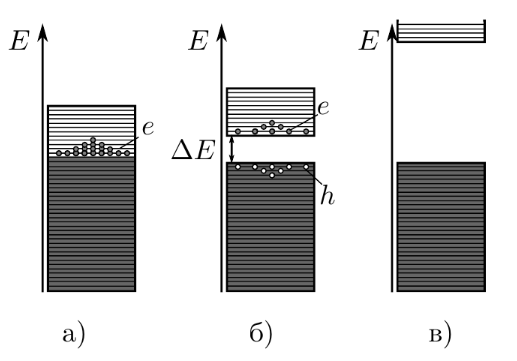
\includegraphics[width=0.5\linewidth]{3.3.4_1.png}
\text{Рис. 1. Структура состояний а) проводника, б) полупроводника, в) диэлектрика}\\
\end{center}

\subsection{Закон Ома}
\hfill \break При наложении внешнего электрического поля \textit{\textbf{E}} носители заряда начинают двигаться ускоренно. Однако после некоторого свободного пробега происходит взаимодействие с решеткой: частица теряет приобретенный импульс и процесс ускорения начинается заново. В результате баланса ускоряющей силы и трения о решетку частица приобретает некоторую среднюю установившуюся скорость дрейфа, пропорциональную приложенному полю:

\begin{equation}\label{ linkname }
\textit{\textbf{u}}_\text{др} = \mu\textit{\textbf{E}}.
\end{equation}

\hfill \break Коэффициент $\mu$ называется \textit{подвижностью} носителя тока. Его знак определяется знаком зарядов (у электронов подвижность отрицательна, у дырок $-$ положительна). Усредненное взаимодействие носителя заряда с кристаллической решеткой можно моделировать действующей на него постоянной силой трения, пропорциональной средней средней скорости \textit{\textbf{u}} его движения:

\begin{equation}\label{ linkname }
\textit{\textbf{F}}_\text{тр} = -\frac{q\textit{\textbf{u}}}{\mu}.
\end{equation}

\hfill \break При концентрации носителей $n$ плотность тока равна

\begin{equation}\label{ linkname }
\textit{\textbf{j}} = qn\textit{\textbf{u}} = qn\mu\textit{\textbf{E}}.
\end{equation}

\hfill \break Коэффициент пропорциональности между \textit{\textbf{j}} и \textit{\textbf{E}} называют \textit{проводимостью} среды. Соответствующую связь

\begin{equation}\label{ linkname }
\textit{\textbf{j}} = \sigma\textit{\textbf{E}}
\end{equation}

\hfill \break называют \textit{законом Ома в дифференциальной форме}. Видно, что проводимость связана с подвижностью как $\sigma = qn\mu$.

\subsection{Эффект Холла}
\hfill \break Во внешнем магнитном поле \textit{\textbf{B}} на заряды действует сила Лоренца:

\begin{equation}\label{ linkname }
\textit{\textbf{F}} = q\textif{\textit{E}} + q\textit{\textbf{u}} \times \textit{\textbf{B}}.
\end{equation}

\hfill \break Эта сила вызывает движение носителей, направление которого в общем случае не совпадает с \textif{\textbf{E}}. Траектории частиц будут либо искривляться, либо возникнет дополнительное электрическое поле, компенсирующее магнитную составляющую силы Лоренца. Возникновение поперечного току электрического поля в образце, помещенном во внешнее магнитное поле, называют \textit{\textbf{эффектом Холла}}. 

\hfill \break Закон Ома можно записать в виде

\begin{equation}\label{ linkname }
\textif{\textbf{j}} = \hat{\sigma}\textit{\textbf{E}},
\end{equation}

\hfill \break если под $\hat{\sigma}$ понимать \textit{тензор проводимости}. В заданном базисе он представляется матрицей $3 \times 3$. Тензорная связь между полем и током имеет место в общем случае, когда проводящая среда не является изотропной. В условиях эффекта Холла тензор проводимости становится недиагональным. \textit{Тензор удельного сопротивления} $\hat{\rho}$ вводится как обратный к тензору проводимости. В условиях эффекта Холла тензор проводимости получается равен

\begin{equation}\label{ linkname }
\hat{\sigma} = \hat{\rho}^{-1} = \frac{\sigma_{0}}{1 + (\mu B)^2} \cdot \begin{pmatrix}
1 & \mu B & 0\\
-\mu B & 1 & c\\
0 & 0 & 1
\end{pmatrix}
\end{equation}

\hfill \break Безразмерному параметру $\mu B$ соответствует отношение эффективной длины пробега частиц $l = \mu mu/q$ к ларморовскому радиусу кривизны их траектории $r_{B} = mu/qB$. Эту величину называют \textit{параметром замагниченности}. 

\subsection{Мостик Холла}
\hfill \break Мостик Холла используется для исследования зависимости проводимости среды от магнитного поля. В данной схеме (рис. 2) ток вынуждают течь по оси $x$ вдоль поской пластинки (ширина пластинки $a$, толщина $h$, длина $l$). Сила Лоренца, действующая со стороны перпендикулярного пластинке магнитного поля, прибивает носители заряда к краям образца, что создает холловское электрическое поле, компенсирующее эту силу. Поперечное напряжение между краями пластинки (холловское напряжение) равно $U_{\perp} = E_{y}a$, где $E_{y} = \frac{j_{x}B}{nq}$.

\begin{wrapfigure}{r}{0.5\textwidth}
\begin{center}
    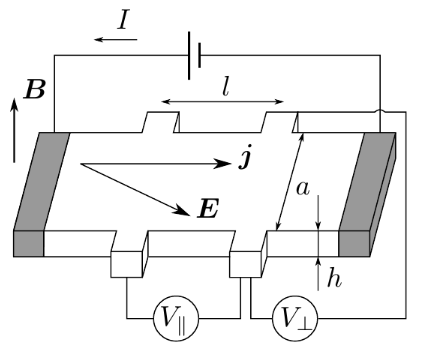
\includegraphics[width=1\textwidth]{3.3.4_2.png}
    \text{Рис. 2. Мостик Холла}
\end{center}
\end{wrapfigure}

\hfill \break Плотность тока, текущего через образец, равна $j_{x} = I/ah$, где $I$ $-$ полный ток, $ah$ $-$ поперечное сечение. Таким образом, для холловского напряжения имеем

\begin{equation}\label{ linkname }
U_{\perp} = \frac{B}{nqh} \cdot I = R_\text{н} \cdot \frac{B}{h} \cdot I,
\end{equation}

\hfill \break где константу $R_\text{н} = \frac{1}{nq}$ называют \textit{константой Холла}, ее знак определяется знаком носителей заряда.

\hfill \break Продольная напряженность электрического поля равна 

$$
E_{x} = \rho_{xx} \cdot j_{x} = j_{x}/\sigma_{0},
$$

\hfill \break где $\sigma_{0} = qn\mu$ $-$ удельная проводимость среды в отсутствие \textit{\textbf{B}}, и падение напряжения $U_{||} = E_{x}l$ вдоль пластинки определяется омическим сопротивлением образца $R_{0} = l/(\sigma_{0}ah)$:

\begin{equation}\label{ linkname }
U_{||} = IR_{0}.
\end{equation}

\section{Экспериментальная установка}
\hfill \break Экспериментальная установка показана на рисунке 3. В зазоре электромагнита создается постоянное магнитное поле, величину которого можно менять с помощью регулятора источника питания электромагнита. Ток питания электромагнита измеряется амперметром $A_{1}$, направление тока в обмотках электромагнита меняется переключением разъема $K_{1}$.

\hfill \break Градуировка магнита проводится при помощи милливеберметра.

\begin{center}
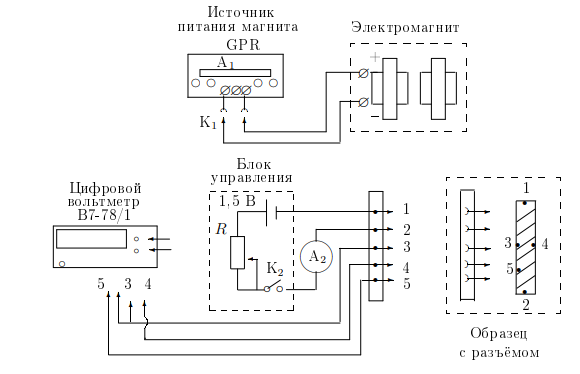
\includegraphics[width=0.6\linewidth]{3.3.4_3.png}
\text{Рис. 3. Схема установки для исследования эффекта Холла в полупроводниках}\\
\end{center}

\hfill \break Образец из легированного германия подключается к батарее. При замыкании ключа $K_{2}$ вдоль длинной стороны образца течет ток, величина которого регулируется реостатом R и измеряется миллиамперметром $A_{2}$. В образце с током, помещенном в зазор электромагнита, между контактами 3 и 4 возникает разность потенциалов $U_{34}$, которая измеряется с помощью цифрового вольтметра. Контакты 3 и 4 вследствие неточности пайки не всегда лежат на одной эквипотенциале, и тогда напряжение между ними связано не только с эффектом Холла, но и с омическим падением напряжения, вызванным протеканием основного тока через образец. Можно исключить влияние омического падения напряжения, если при каждом токе через образец измерять напряжение между точками 3 и 4 в отсутствие магнитного поля. При фиксированном токе через образец это дополнительное к ЭДС Холла напряжение $U_{0}$ остается неизменным, тогда ЭДС Холла: 

\begin{equation}\label{ linkname }
\mathcal{E}_{x} = U_{34} \pm U_{0}. 
\end{equation}

\hfill \break По знаку $\mathcal{E}_{x}$ можно определить характер проводимости $-$ электронный или дырочный. Для этого необходимо знать направление тока в образце и направление магнитного поля.

\hfill \break Измерив ток I в образце и напряжение $U_{35}$ между контактами 3 и 5 в отсутствие магнитного поля, можно, зная параметры образца, рассчитать проводимость материала по формуле:

\begin{equation}\label{ linkname }
\sigma = \frac{I \cdot L_{35}}{U_{35} \cdot a \cdot l},
\end{equation}

\hfill \break где $L_{35}$ $-$ расстояние между контактами 3 и 5, $a$ $-$ толщина образца, $l$ $-$ его ширина.

\section{Ход работы}
\hfill \break В работе предлагается исследовать зависимость ЭДС Холла от величины магнитного поля при различных токах через образец для определения константы Холла, определить знак носителей заряда и проводимость материала образца. Подготовим все приборы к работе согласно описанию на установке.

\subsection{Градуировка электромагнита}
\hfill \break Проведем калибровку электромагнита $-$ определим связь между индукцией магнитного поля в зазоре электромагнита и током через обмотку магнита. Для этого снимем зависимость магнитного потока Ф, пронизывающего катушку в поле, от тока $I_\text{м}$ и найдем величину магнитной индукции по формуле:

$$
B = \frac{\Delta \text{Ф}}{SN},
$$

\hfill \break где $\Delta \text{Ф} = \text{Ф} - \text{Ф}_{0}$ $-$ разность между конечным и начальным значениями потока вектора индукции, который пронизывал пробную катушку, находившуюся в зазоре электромагнита. Значение $(SN)$ $-$ 72 $\text{см}^2 \cdot \text{вит}$. Результаты занесем в таблицу 1, а также отобразим на графике полученную калибровочную кривую (рис. 4):

\begin{center}
\begin{tabular}{|c|c|c|c|}\hline
$I_\text{м}$, A&$\Delta \text{Ф}$, мВб&$B$, мТл&$\sigma B$, мТл\\\hline
$0.00$&$0.20$&$27.78$&$0.28$\\\hline
$0.26$&$1.60$&$222$&$2$\\\hline
$0.50$&$3.00$&$417$&$4$\\\hline
$0.75$&$4.30$&$597$&$6$\\\hline
$1.00$&$5.50$&$764$&$8$\\\hline
$1.25$&$6.60$&$917$&$9$\\\hline
$1.50$&$7.30$&$1014$&$10$\\\hline
$1.75$&$7.80$&$1083$&$11$\\\hline
$1.96$&$8.20$&$1139$&$11$\\\hline
$2.00$&$8.20$&$1139$&$11$\\\hline
\end{tabular}\\
\hfill \break \textbf {Таблица 1.} Исследование зависимости индукции магнитного поля от тока через обмотку\\
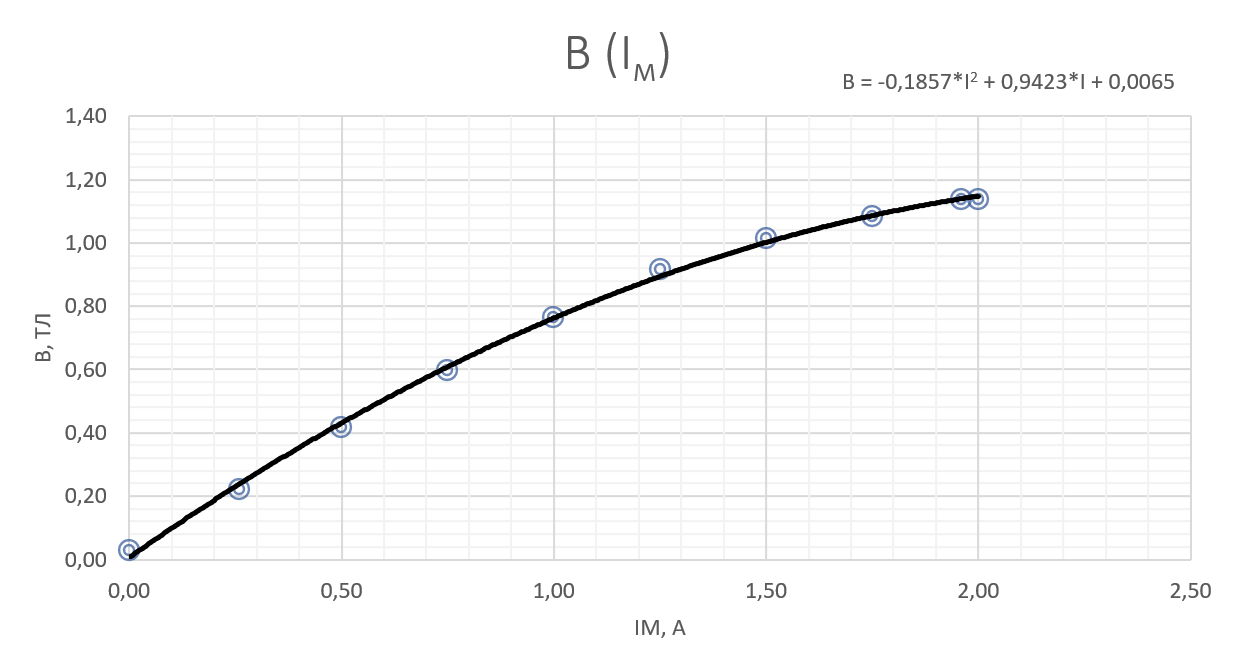
\includegraphics[width=0.95\textwidth]{3.3.4_4.png}\\
\textbf{Рис. 4.} График зависимости $B$ ($I_\text{м}$)~\\
\end{center}

\hfill \break Уравнение полученной зависимости показано на рисунке. Нам достаточно знать конечный набор значений магнитного поля и проводить измерения $U_{34}$ на них. Также зафиксируем погрешности некоторых измеряемых величин (таблица 2) и параметры установки (таблица 3).

\begin{center}
\begin{tabular}{|c|c|c|c|c|}\hline
&$\text{Ф}$, мВб&$I_\text{м}$, А&$U_{34}$, мкВ&$I$, мА\\\hline
$\text{Величина}$&$1$&$1$&$50$&$0.5$\\\hline
$\text{Погрешность}, \sigma$&$0.01$&$0.01$&$1$&$0.005$\\\hline
$\varepsilon$, $\%$&$1$&$1$&$2$&$1$\\\hline
\end{tabular}\\
\hfill \break \textbf {Таблица 2.} Погрешности некоторых измеряемых величин\\~\\
\end{center}

\hfill \break

\begin{center}
\begin{tabular}{|c|c|c|}\hline
$L_{35}$, мм&$3.0$\\\hline
$a$, мм&$1.5$\\\hline
$l$, мм&$1.7$\\\hline
\end{tabular}\\
\hfill \break \textbf {Таблица 3.} Параметры установки\\~\\
\end{center}

\subsection{Измерение ЭДС Холла}
\hfill \break Проведем измерение ЭДС Холла. Сначала вставим в зазор выключенного электромагнита образец, параметры которого зафиксированы в таблице 3, и определим напряжение $U_{0}$ между холловскими контактами 3 и 4 при минимальном токе через образец. Это напряжение вызвано несовершенством контактов 3, 4 и при фиксированном токе остается неизменным $-$ примем его за начало отсчета.  

\hfill \break Затем снимем зависимость напряжения $U_{34}$ от тока электромагнита $I_\text{м}$ при фиксированном токе $I$ через образец. Повторим эти действия для различных токов через образец. Также каждое значение тока электромагнита мы можем сопоставить со значением индукции магнитного поля в зазоре электромагнита, измеренным при калибровке. При максимальном токе через образец проведем еще измерения при обратном направлении магнитного поля. 

\hfill \break Результаты измерений занесем в таблицу 4, а также построим на одном графике семейство зависимостей ЭДС Холла от магнитного поля в электромагните при различных токах через образец. 

\begin{center}
\begin{tabular}{|c|c|c|c|c|c|c|c|c|c|}\hline
$I_\text{м}$, A&$0.00$&$0.25$&$0.50$&$0.75$&$1.00$&$1.25$&$1.50$&$1.75$&$2.00$\\\hline
$B$, мТл&$27.78$&$222$&$417$&$597$&$764$&$917$&$1014$&$1083$&$1139$\\\hline
$U_{34}$$(0.3 \text{мA})$&$-0.018$&$0.004$&$0.026$&$0.049$&$0.067$&$0.083$&$0.095$&$0.104$&$0.110$\\\hline
$U_{34}$$(0.4 \text{мA})$&$-0.023$&$0.005$&$0.036$&$0.066$&$0.091$&$0.114$&$0.130$&$0.140$&$0.148$\\\hline
$U_{34}$$(0.5 \text{мA})$&$-0.028$&$0.006$&$0.045$&$0.080$&$0.113$&$0.140$&$0.160$&$0.173$&$0.184$\\\hline
$U_{34}$$(0.6 \text{мA})$&$-0.035$&$0.010$&$0.055$&$0.097$&$0.136$&$0.170$&$0.194$&$0.210$&$0.223$\\\hline
$U_{34}$$(0.7 \text{мA})$&$-0.040$&$0.010$&$0.063$&$0.115$&$0.159$&$0.197$&$0.226$&$0.246$&$0.260$\\\hline
$U_{34}$$(0.8 \text{мA})$&$-0.047$&$0.010$&$0.072$&$0.133$&$0.183$&$0.228$&$0.258$&$0.281$&$0.297$\\\hline
$U_{34}$$(0.9 \text{мA})$&$-0.053$&$0.012$&$0.080$&$0.147$&$0.205$&$0.255$&$0.291$&$0.316$&$0.334$\\\hline
$U_{34}$$(1.0 \text{мA})$&$-0.059$&$0.016$&$0.091$&$0.164$&$0.230$&$0.283$&$0.324$&$0.352$&$0.374$\\\hline
$U_{34}$$(1.0 \text{мA})$&$-0.071$&$-0.140$&$-0.218$&$-0.292$&$-0.361$&$-0.423$&$-0.470$&$-0.497$&$-0.520$\\\hline
\end{tabular}\\
\hfill \break \textbf {Таблица 4.} Зависимость напряжения $U_{34}$ [В] от тока электромагнита $I_\text{м}$ при фиксированном токе $I$ через образец\\
\end{center}

\hfill \break Построим график зависимости ЭДС Холла от величины магнитной индукции при разных значениях тока через образец $I$ и определим угловые коэффициенты получившихся прямых. ЭДС Холла определяется по формуле (10).

\begin{center}
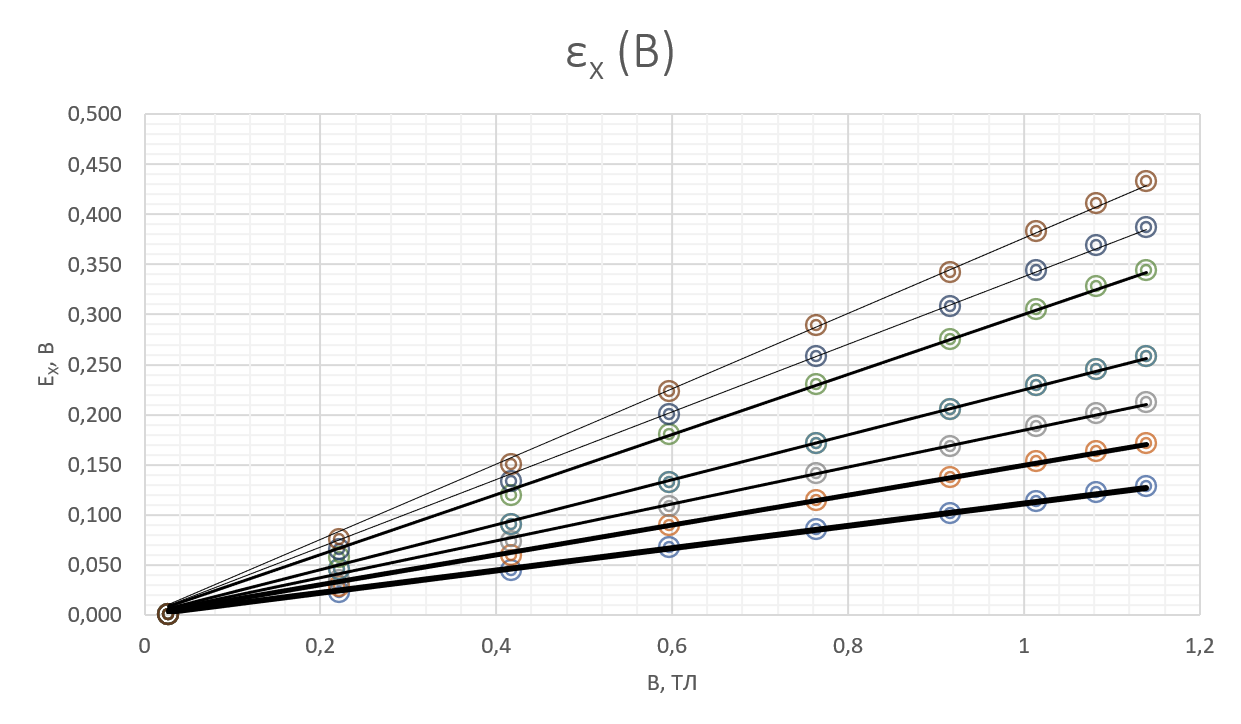
\includegraphics[width=0.95\textwidth]{3.3.4_5.png}\\
\textbf{Рис. 5.} График зависимости $\varepsilon_{x}$ ($B$)~\\
\end{center}

\hfill \break Здесь самая верхняя прямая соответствует $I = 1.0$А, самая нижняя $-$ $I = 0.3$А. Для каждой прямой рассчитаем значение коэффициента наклона по формуле $k = d\varepsilon_{x}/dB$ и построим график $k(I)$:

\begin{center}
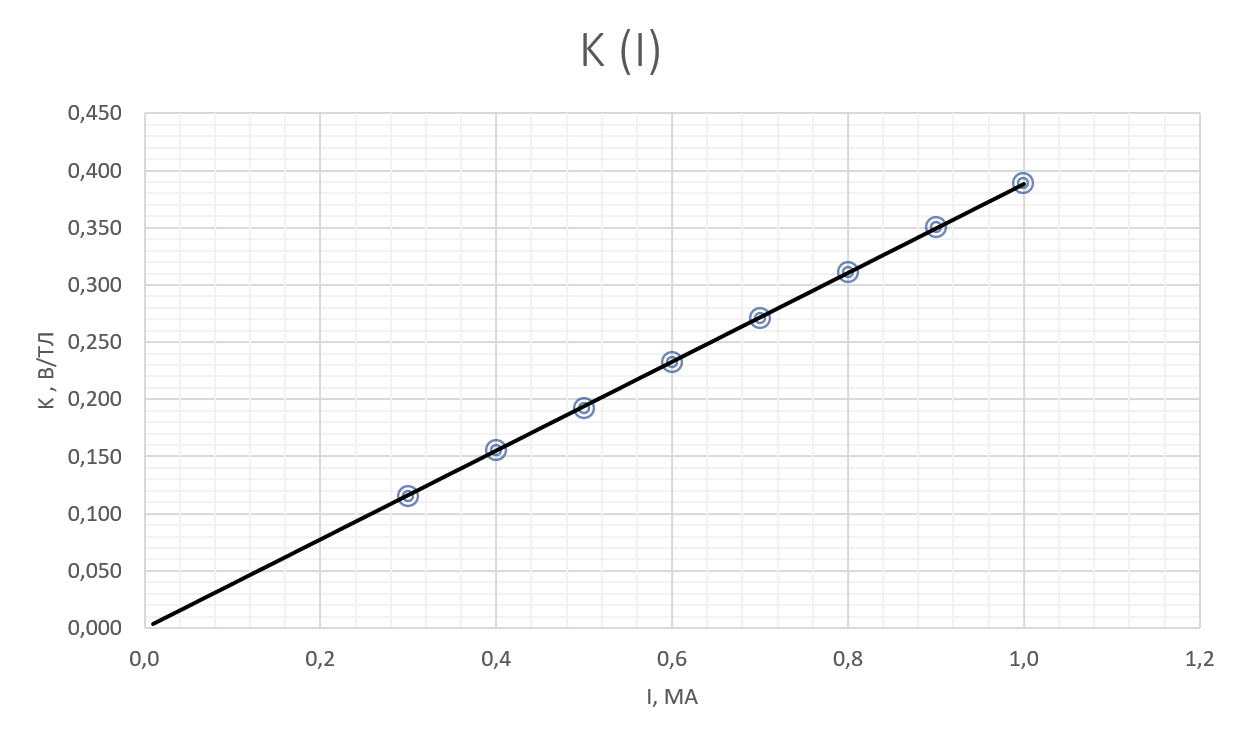
\includegraphics[width=0.95\textwidth]{3.3.4_6.png}\\
\textbf{Рис. 6.} График зависимости $k$ ($I$)~\\
\end{center}

\hfill \break Рассчитаем размерность $k$: $k = \frac{\varepsilon_{x}}{B}$, где $[\varepsilon_{x}] = [\text{В}]$, а $[B] = [\text{Тл}]$, то есть $[k] = [\text{В/Тл}]$. Коэффициент наклона последнего графика $-$ $K = 0.391 = k / I$. Относительная погрешность определения этого коэффициента с учетом метода наименьших квадратов и систематических погрешностей получилась порядка 10\%. Теперь можем найти значение \textit{постоянной Холла} при помощи формулы (8). 

$$
R_\text{н} = \frac{\varepsilon_{x} \cdot a}{B \cdot I} = k \cdot \frac{a}{I} = K \cdot a = (0.665 \pm 0.080) \cdot 10^{-3}  \text{ м}^{3}/\text{Кл}.
$$

\hfill \break Рассчитаем \textit{концентрацию носителей тока}:

$$
n = \frac{1}{R_\text{н}e} = (9.40 \pm 1.13)\cdot 10^{21}\text{ ед}/\text{м}^3.
$$

\subsection{Определение характера проводимости}
\hfill \break Определим характер проводимости в образце. Направление тока через образец и направление магнитного поля показаны стрелками на рисунке 7:

\begin{center}
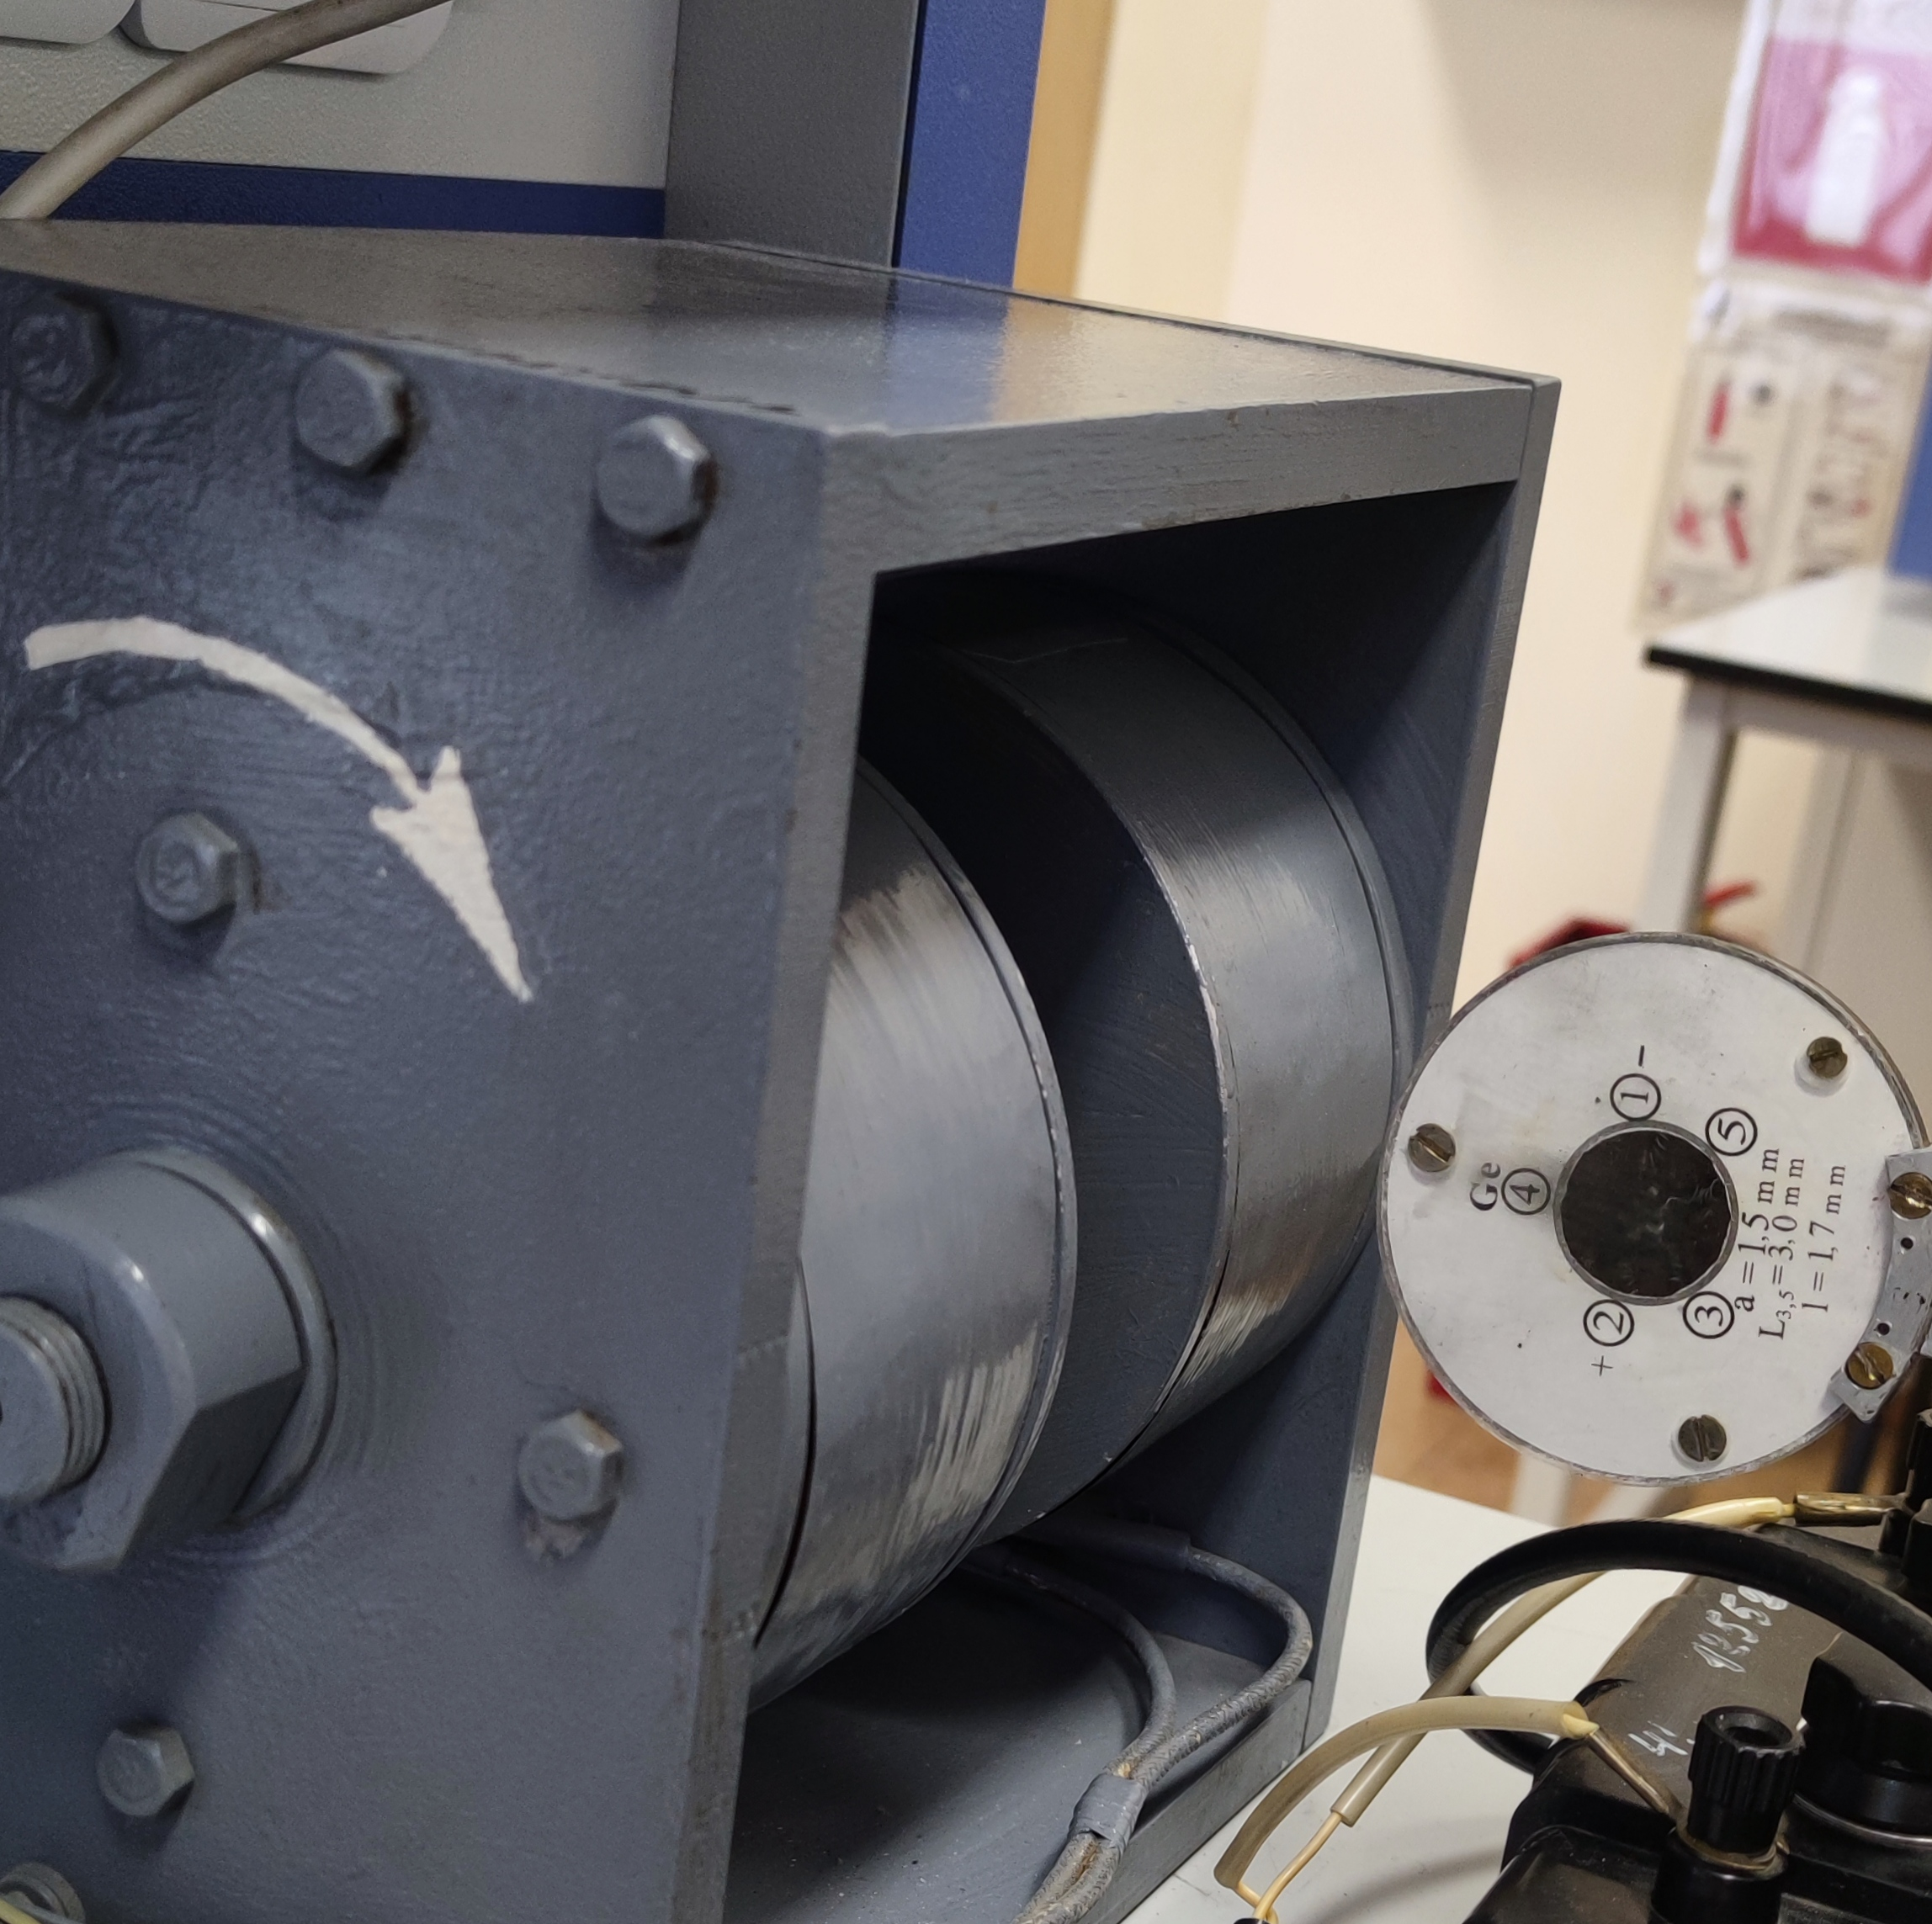
\includegraphics[width=0.7\textwidth]{3.3.4_7.jpg}\\
\textbf{Рис. 7.} Установка~\\
\end{center}

\hfill \break Зная направление магнитного поля в электромагните и тока через образец, можно определить, что носители тока заряжены отрицательно, то есть проводимость \textit{электронная}.

\subsection{Определение удельной проводимости}
\hfill \break По формуле (11) рассчитаем удельную проводимость исследуемого образца. Для этого выключим источник питания электромагнита и удалим держатель с образцом из зазора. При токе через образец $I = 1$мА измерим падение напряжения $U_{35}$ и определим \textit{проводимость}:

$$
\sigma = \frac{I \cdot L_{35}}{U_{35} \cdot a \cdot l} = (153.9 \pm 0.8) \frac{1}{\text{Ом} \cdot \text{м}}.
$$

\hfill \break Из полученных значений можно вывести \textit{подвижность} носителей тока (электронов):

$$
b = \frac{\sigma}{ne} = \sigma R_\text{н} = (1446 \pm 245) \frac{\text{см}^2}{\text{В} \cdot \text{с}}.
$$

\hfill \break Табличное значение подвижности для электронной проводимости $-$ $b_\text{теор} = 3800 \frac{\text{см}^2}{\text{В} \cdot \text{с}}.$

\section{Вывод}
\hfill \break В работе проводилось исследование эффекта Холла на примере полупроводника $-$ легированного германия. Для него были определены постоянная Холла, концентрация холловских частиц, удельная проводимость и подвижность носителей зарядов. Полученные значения совпали с табличными хотя бы по порядку величины. Погрешность вычислений оказалась достаточно значительной, что может быть связано с вероятно большим количеством примесей в исследуемом веществе или с тем, что характер проводимости в исследуемом образце не чисто электронный, а электронно-дырочный.

\end{document}
